% windsor's engineering notepad template
% uses emerald and lxfonts packages from ctan
%
% don't forget to change the date and other info in the header!!
%
% convert to bitmap with:
% convert -density 300x300 notes_template.pdf -resize 800x notes_template.png

\documentclass[12pt]{article}
\usepackage{CJK}
\usepackage[T1]{fontenc}
\usepackage{amsfonts}
\usepackage{emerald}
\usepackage{lxfonts}
\usepackage{amsmath}
\usepackage{graphicx}
\usepackage{eso-pic}
\usepackage{lastpage}
\usepackage[left=2.7cm,right=1.7cm,top=1.65cm,bottom=1.0cm]{geometry}




%��������������
\usepackage{mdframed}
\usepackage{enumerate}
\usepackage{multirow}

%����eps
\usepackage{graphicx}
\usepackage{epstopdf}
\usepackage{subfigure}

%������ַ
\usepackage{url}

%���볬����
\usepackage[colorlinks,linkcolor=blue]{hyperref}











% configure page header
\usepackage{fancyhdr}
\setlength{\headheight}{15pt}
\pagestyle{fancy}\fancyhf{}
\renewcommand{\headrulewidth}{0pt}
\renewcommand{\footrulewidth}{0pt}
\lhead{\normalfont\ECFAugie \large{\MakeUppercase{07/24/17}}}
\chead{\normalfont\ECFAugie \large{Y. C}\hspace{1.4cm}}
\rhead{\normalfont\ECFAugie \large{\hspace{1cm} Convex Opt. NOTES}\hspace{0.5cm}\thepage\hspace{0.1cm}/\hspace{0.1cm}\pageref{LastPage}\hspace{-1.5cm}}

% background image
\newcommand\BackgroundPic{
\put(0,0){
\parbox[b][\paperheight]{\paperwidth}{%
\vfill
\centering
\includegraphics[width=\paperwidth,height=\paperheight,
keepaspectratio]{background.png}%
\vfill
}}}

% configure section titles
\usepackage{titlesec}
\titleformat{\section}{\Large}{\thesection}{1em}{}
\titleformat{\subsection}{\large\bfseries}{\thesubsection}{1em}{}

\begin{document}
\begin{CJK*}{GBK}{song}
\AddToShipoutPicture{\BackgroundPic}
\normalfont\ECFAugie

% custom commands
\newcommand{\windef}[1]{\subsection*{\underline{DEF:} \normalsize{#1}}} % definition
\newcommand{\winex}[1]{\subsection*{\underline{EX:} \normalsize{#1}}} % example
\newcommand{\winsec}[1]{\section*{\underline{#1}}} % section
\newcommand{\winres}[1]{\begin{math}\Rightarrow\left\{\begin{matrix}#1\end{matrix}\right.\end{math}\hspace{0.2cm}} % result
\newcommand{\winsys}[1]{\begin{math}\left\{\begin{matrix}#1\end{matrix}\right.\end{math}} % system
\newcommand{\winero}[1]{\begin{math}\xrightarrow{#1}\end{math}} % row operation
\newcommand{\winmat}[1]{\begin{math}\begin{bmatrix}#1\end{bmatrix}\end{math}} % matrix
\newcommand{\winsub}[1]{\subsection*{$\star$\hspace{0.2cm} #1}} % dot
\newcommand{\step}[1]{\begin{math}\xrightarrow{\text{#1}}\end{math}} % step in a process
\newcommand{\winrtwo}{\begin{math}\text{R}^\text{2}\end{math}}
\newcommand{\winrthree}{\begin{math}\text{R}^\text{3}\end{math}}
\newcommand{\wineq}[1]{\begin{equation}\notag#1\end{equation}}

%%%%%%%%%%%%%%%%%%%%%%
% start writing here %
%%%%%%%%%%%%%%%%%%%%%%


\section{Foundation}
\subsection{Introduction}
\winsub{(mathematical) optimization problem}

\begin{table}[!htb]
	\begin{center}

		\begin{tabular}{l l}
			   {\rm minimize} & $f_0(x)$\\
                {\rm subject to}  & $f_i(x)\leq b_i,i=1,\dots,m$
		\end{tabular}
	\end{center}
\end{table}
\begin{itemize}
    \item $x=(x1,\dots,x_n)$: optimization variables 
    \item $f_0: {\bf R}^n \rightarrow {\bf R}$: objective function
    \item $f_i: {\bf R}^n \rightarrow {\bf R}, i=1,\dots,m$: constraint functions
\end{itemize}

{\bf optimal solution} $x^*$ has smallest value of $f_0$ among all vectors that satisfy the constaints

\winex{portfolio optimization}
\begin{itemize}
\item variables: amounts invested in different assets
\item constraints: budget, {\rm max./min.} investment per asset, minimum return
\item object: overall risk or return variance
\end{itemize}

\winex{data fitting}
\begin{itemize}
\item variables: model parameters
\item constraints: prior information, parameter limits
\item objective: measure of misfit or prediction error
\end{itemize}

\winsub{Least-squares}
\begin{table}[!htb]
	\begin{center}

		\begin{tabular}{c c}
			   {\rm minimize} & $\|Ax-b\|_2^2$
		\end{tabular}
	\end{center}
\end{table}
{\bf solving least-squares problems}
\begin{itemize}
\item analytical solution: $x^{*}=(A^TA)^{-1}A^Tb$
\item reliable and efficient algorithms and software
\item computation time proportional to $n^2k$ ($A\in {\bf R}^{k\times n}$); less if structured
\item a mature technology
\end{itemize}

{\bf using least-squares}
\begin{itemize}
\item least-squares problems are easy to recognize
\item a few standard techniques increase flexibility (e.g., including weights, adding regularization terms)
\end{itemize}

\winsub{Linear programming}
\begin{table}[!htb]
	\begin{center}

		\begin{tabular}{l l}
			   {\rm minimize} & $c^Tx$ \\
                {\rm subject to} & $a_i^Tx\leq b_i, i=1,\dots,m$
		\end{tabular}
	\end{center}
\end{table}
{\bf solving linear programs}
\begin{itemize}
\item no analytical formula for solution
\item reliable and efficient algorithms and software
\item computation time proportional to $n^2m$ if $m \geq n$; less with structure
\item a mature technology
\end{itemize}

{\bf using linear programming}
\begin{itemize}
\item not as easy to recognize as least-squares problems
\item a few standard tricks used to convert problems into linear programs (e.g., problems involving $l_1-$ or $l_\infty-$norms, piecewise-linear functions)
\end{itemize}

\winsub{Convex optimization problem}
\begin{table}[!htb]
	\begin{center}

		\begin{tabular}{l l}
			   {\rm minimize} & $f_0(x)$\\
                {\rm subject to}  & $f_i(x)\leq b_i,i=1,\dots,m$
		\end{tabular}
	\end{center}
\end{table}
\begin{itemize}
\item objective and constraint functions are convex 
    $$f_i(\alpha x+\beta y)\leq \alpha f_i(x)+\beta f_i(y)$$
    if $\alpha+\beta =1, \alpha \geq 0, \beta \geq 0$
\item includes least-squares problems and linear programs as special cases
\end{itemize}

{\bf solving convex optimization problems}
\begin{itemize}
\item no analytical solution
\item reliable and efficient algorithms
\item computation time (roughly) proportional to $\max{\{n^3, n^2m, F\}}$, where $F$ is cost of evaluating $f_i$'s and their first and second derivatives
\item almost a technology
\end{itemize}

{\bf using convex optimization}
\begin{itemize}
\item often difficult to recognize
\item many tricks for transforming problems into convex form
\item surprisingly many problems can be solved via convex optimization
\end{itemize}

\subsection{Convex sets}
\winsub{Affine set}
{\bf line} through $x_1$,$x_2$: all pints
$$x=\theta x_1+(1-\theta)x_2\indent  (\theta \in {\bf R})$$
\begin{figure}[!htb]
\centering
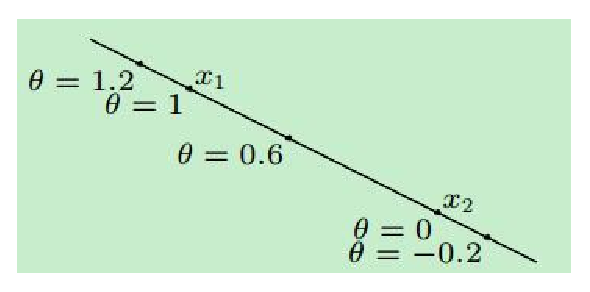
\includegraphics[width=0.3\columnwidth ]{line.eps}
\end{figure}

\windef{affine set}
{\bf affine set}: contains the line through any two distinct points in the set

\winsub{Convex set}
{\bf line segment} between $x_1$ and $x_2$: all points
$$x=\theta x_1+(1-\theta)x_2$$
with $0\leq \theta \leq 1$

\windef{convex set}
{\bf convex set}: contains line segment between any two points in the set
$$x_1,x_2\in C, 0\leq \theta \leq 1 \Rightarrow \theta x_1+(1-\theta)x_2\in C$$

\winsub{Convex combination and convex hull}
\windef{convex combination}
{\bf convex combination} of $x_1,\dots,x_k$: any point $x$ of the form
$$x=\theta_1 x_1+\theta_2 x_2+\dots+\theta_k x_k$$
with $\theta_1+\dots+\theta_k=1,\theta_i|geq0$
\windef{convex hull conv $S$}
{\bf convex hull conv $S$}: set of all combinations of points in $S$

\winsub{Convex cone}
\windef{conic (nonnegative) combination}
{\bf conic (nonnegative) combination} of $x_1$ and $x_2$: any point of the form
$$x=\theta_1 x_1+\theta_2 x_2$$
withe $\theta_1\geq 0, \theta_2 \geq 0$
\begin{figure}[!htb]
\centering
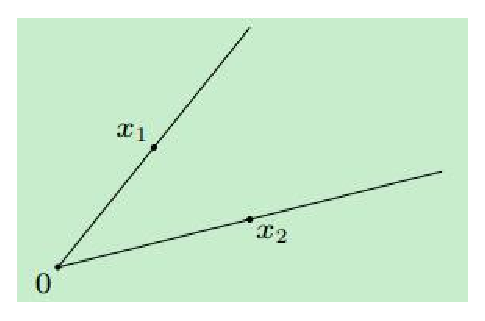
\includegraphics[width=0.3\columnwidth ]{conicCombination.eps}
\end{figure}
\windef{convex cone}
{\bf convex cone}: set that contains all conic combinations of points in the set

\winsub{Hyperplanes and halfspaces}
\windef{hyperplane}
{\bf hyperplane}: set of the form $\{x|a^Tx=b\}\indent (a\neq 0)$
\begin{figure}[!htb]
\centering
\includegraphics[width=0.3\columnwidth ]{hyperplane}
\end{figure}

\windef{halfspace}
{\bf halfspace}: set of the form $\{x|a^Tx\leq b\}\indent (a\neq 0)$
\begin{figure}[!htb]
\centering
\includegraphics[width=0.3\columnwidth ]{halfspace}
\end{figure}

{\bf remark}
\begin{itemize}
\item $a$ is the normal vector
\item hyperplanes are affine and convex; halfspaces are convex
\end{itemize}








\begin{table}[!htb]
	\begin{center}

		\begin{tabular}{l l}
                $   $ & $  $\\
			   $   $ & $  $\\
                $   $ & $  $\\
			   $   $ & $  $\\
                $   $ & $  $\\
			   $   $ & $  $\\
                $   $ & $  $\\
			   $   $ & $  $\\
                $   $ & $  $\\
			   $   $ & $  $\\
                $   $ & $  $\\
			   $   $ & $  $\\
                $   $ & $  $\\
			   $   $ & $  $\\
                $   $ & $  $\\
			   $   $ & $  $\\
                $   $ & $  $\\
			   $   $ & $  $\\
                $   $ & $  $\\
			   $   $ & $  $\\
                $   $ & $  $\\
			   $   $ & $  $\\
                $   $ & $  $\\
			   $   $ & $  $\\
                $   $ & $  $\\
			   $   $ & $  $\\
                $   $ & $  $\\
			   $   $ & $  $\\
                $   $ & $  $\\
			   $   $ & $  $\\
                $   $ & $  $\\
			   $   $ & $  $\\
                $   $ & $  $\\
			   $   $ & $  $\\
		\end{tabular}
	\end{center}
\end{table}



% section
\winsec{section name goes here}

% term definition
\winsub{term definition}
\windef{term - and it's definition}

% example
\winsub{an example}
\winex{example heading}

% system of equations
\winsub{a system of equations}
\winsys{
2x+4y=2 \\
2x+6y=3}

% matrix
\winsub{working a multistep problem}
\winmat{
a & b & c \\
d & e & f \\
g & h & i }
% row operation
\winero{R_1+R_2}
% matrix
\winmat{
a & b & c \\
d & e & f \\
g & h & i }
% result
\winres{
x = 1 \\
y = 2 \\
z = 3}

% vector in 3-space
\winsub{a vector in \winrthree}
v = \winmat{
x \\
y \\
z }

\winsub{a multi-step process}
A \step{do stuff} B \step{more stuff} C

% numbered list
\winsub{an enumerated list}
\begin{enumerate}
\item{this is the first item in an enumerated list}
\item{this is the second item in an enumerated list}
\end{enumerate}

% manual line breaks
\winsub{manually broken lines}
the first line\\
the second line\\
the third line

% equation
\winsub{some math}
\wineq{
\int_a^b \! f(x) \; dx % definite
\int \! f(x) \, dx \; % indefinite
\frac{\pi}{2} \; % fraction
\sqrt{\theta} \; % root
n = 1,2,3 \ldots 4}



\end{CJK*}
\end{document}
